\documentclass{ximera}

 

\usepackage{epsfig}

\graphicspath{
  {./}
  {figures/}
}

\usepackage{morewrites}
\makeatletter
\newcommand\subfile[1]{%
\renewcommand{\input}[1]{}%
\begingroup\skip@preamble\otherinput{#1}\endgroup\par\vspace{\topsep}
\let\input\otherinput}
\makeatother

\newcommand{\includeexercises}{\directlua{dofile("/home/jim/linearAlgebra/laode/exercises.lua")}}

%\newcounter{ccounter}
%\setcounter{ccounter}{1}
%\newcommand{\Chapter}[1]{\setcounter{chapter}{\arabic{ccounter}}\chapter{#1}\addtocounter{ccounter}{1}}

%\newcommand{\section}[1]{\section{#1}\setcounter{thm}{0}\setcounter{equation}{0}}

%\renewcommand{\theequation}{\arabic{chapter}.\arabic{section}.\arabic{equation}}
%\renewcommand{\thefigure}{\arabic{chapter}.\arabic{figure}}
%\renewcommand{\thetable}{\arabic{chapter}.\arabic{table}}

%\newcommand{\Sec}[2]{\section{#1}\markright{\arabic{ccounter}.\arabic{section}.#2}\setcounter{equation}{0}\setcounter{thm}{0}\setcounter{figure}{0}}

\newcommand{\Sec}[2]{\section{#1}}

\setcounter{secnumdepth}{2}
%\setcounter{secnumdepth}{1} 

%\newcounter{THM}
%\renewcommand{\theTHM}{\arabic{chapter}.\arabic{section}}

\newcommand{\trademark}{{R\!\!\!\!\!\bigcirc}}
%\newtheorem{exercise}{}

\newcommand{\dfield}{{\sf dfield9}}
\newcommand{\pplane}{{\sf pplane9}}

\newcommand{\EXER}{\section*{Exercises}}%\vspace*{0.2in}\hrule\small\setcounter{exercise}{0}}
\newcommand{\CEXER}{}%\vspace{0.08in}\begin{center}Computer Exercises\end{center}}
\newcommand{\TEXER}{} %\vspace{0.08in}\begin{center}Hand Exercises\end{center}}
\newcommand{\AEXER}{} %\vspace{0.08in}\begin{center}Hand Exercises\end{center}}

% BADBAD: \newcommand{\Bbb}{\bf}

\newcommand{\R}{\mbox{$\Bbb{R}$}}
\newcommand{\C}{\mbox{$\Bbb{C}$}}
\newcommand{\Z}{\mbox{$\Bbb{Z}$}}
\newcommand{\N}{\mbox{$\Bbb{N}$}}
\newcommand{\D}{\mbox{{\bf D}}}
\usepackage{amssymb}
%\newcommand{\qed}{\hfill\mbox{\raggedright$\square$} \vspace{1ex}}
%\newcommand{\proof}{\noindent {\bf Proof:} \hspace{0.1in}}

\newcommand{\setmin}{\;\mbox{--}\;}
\newcommand{\Matlab}{{M\small{AT\-LAB}} }
\newcommand{\Matlabp}{{M\small{AT\-LAB}}}
\newcommand{\computer}{\Matlab Instructions}
\newcommand{\half}{\mbox{$\frac{1}{2}$}}
\newcommand{\compose}{\raisebox{.15ex}{\mbox{{\scriptsize$\circ$}}}}
\newcommand{\AND}{\quad\mbox{and}\quad}
\newcommand{\vect}[2]{\left(\begin{array}{c} #1_1 \\ \vdots \\
 #1_{#2}\end{array}\right)}
\newcommand{\mattwo}[4]{\left(\begin{array}{rr} #1 & #2\\ #3
&#4\end{array}\right)}
\newcommand{\mattwoc}[4]{\left(\begin{array}{cc} #1 & #2\\ #3
&#4\end{array}\right)}
\newcommand{\vectwo}[2]{\left(\begin{array}{r} #1 \\ #2\end{array}\right)}
\newcommand{\vectwoc}[2]{\left(\begin{array}{c} #1 \\ #2\end{array}\right)}

\newcommand{\ignore}[1]{}


\newcommand{\inv}{^{-1}}
\newcommand{\CC}{{\cal C}}
\newcommand{\CCone}{\CC^1}
\newcommand{\Span}{{\rm span}}
\newcommand{\rank}{{\rm rank}}
\newcommand{\trace}{{\rm tr}}
\newcommand{\RE}{{\rm Re}}
\newcommand{\IM}{{\rm Im}}
\newcommand{\nulls}{{\rm null\;space}}

\newcommand{\dps}{\displaystyle}
\newcommand{\arraystart}{\renewcommand{\arraystretch}{1.8}}
\newcommand{\arrayfinish}{\renewcommand{\arraystretch}{1.2}}
\newcommand{\Start}[1]{\vspace{0.08in}\noindent {\bf Section~\ref{#1}}}
\newcommand{\exer}[1]{\noindent {\bf \ref{#1}}}
\newcommand{\ans}{}
\newcommand{\matthree}[9]{\left(\begin{array}{rrr} #1 & #2 & #3 \\ #4 & #5 & #6
\\ #7 & #8 & #9\end{array}\right)}
\newcommand{\cvectwo}[2]{\left(\begin{array}{c} #1 \\ #2\end{array}\right)}
\newcommand{\cmatthree}[9]{\left(\begin{array}{ccc} #1 & #2 & #3 \\ #4 & #5 &
#6 \\ #7 & #8 & #9\end{array}\right)}
\newcommand{\vecthree}[3]{\left(\begin{array}{r} #1 \\ #2 \\
#3\end{array}\right)}
\newcommand{\cvecthree}[3]{\left(\begin{array}{c} #1 \\ #2 \\
#3\end{array}\right)}
\newcommand{\cmattwo}[4]{\left(\begin{array}{cc} #1 & #2\\ #3
&#4\end{array}\right)}

\newcommand{\Matrix}[1]{\ensuremath{\left(\begin{array}{rrrrrrrrrrrrrrrrrr} #1 \end{array}\right)}}

\newcommand{\Matrixc}[1]{\ensuremath{\left(\begin{array}{cccccccccccc} #1 \end{array}\right)}}



\renewcommand{\labelenumi}{\theenumi)}
\newenvironment{enumeratea}%
{\begingroup
 \renewcommand{\theenumi}{\alph{enumi}}
 \renewcommand{\labelenumi}{(\theenumi)}
 \begin{enumerate}}
 {\end{enumerate}\endgroup}



\newcounter{help}
\renewcommand{\thehelp}{\thesection.\arabic{equation}}

%\newenvironment{equation*}%
%{\renewcommand\endequation{\eqno (\theequation)* $$}%
%   \begin{equation}}%
%   {\end{equation}\renewcommand\endequation{\eqno \@eqnnum
%$$\global\@ignoretrue}}

%\input{psfig.tex}

\author{Martin Golubitsky and Michael Dellnitz}

%\newenvironment{matlabEquation}%
%{\renewcommand\endequation{\eqno (\theequation*) $$}%
%   \begin{equation}}%
%   {\end{equation}\renewcommand\endequation{\eqno \@eqnnum
% $$\global\@ignoretrue}}

\newcommand{\soln}{\textbf{Solution:} }
\newcommand{\exercap}[1]{\centerline{Figure~\ref{#1}}}
\newcommand{\exercaptwo}[1]{\centerline{Figure~\ref{#1}a\hspace{2.1in}
Figure~\ref{#1}b}}
\newcommand{\exercapthree}[1]{\centerline{Figure~\ref{#1}a\hspace{1.2in}
Figure~\ref{#1}b\hspace{1.2in}Figure~\ref{#1}c}}
\newcommand{\para}{\hspace{0.4in}}

\renewenvironment{solution}{\suppress}{\endsuppress}

\ifxake
\newenvironment{matlabEquation}{\begin{equation}}{\end{equation}}
\else
\newenvironment{matlabEquation}%
{\let\oldtheequation\theequation\renewcommand{\theequation}{\oldtheequation*}\begin{equation}}%
  {\end{equation}\let\theequation\oldtheequation}
\fi

\makeatother


\title{mo6.tex}

\begin{document}
\begin{abstract}
BADBAD
\end{abstract}
\maketitle

\chapter{Closed Form Solutions for Planar ODEs}

\subsection*{Section~\protect{\ref{S:6.1}} The Initial Value Problem}
\rhead{S:6.1}{THE INITIAL VALUE PROBLEM}

\exer{c6.1.03a}
\ans The vector $v_1 = (2,-3)^t$ is an eigenvector with associated
eigenvalue $\lambda_1 = 2$.  The vector $v_2 = (-7,11)^t$ is an
eigenvector with associated eigenvalue $\lambda_2 = -1$.

\soln Calculate:
\[
\begin{array}{rcl}
\mattwo{65}{42}{-99}{-64}\vectwo{2}{-3} & = & \vectwo{4}{-6} =
2\vectwo{2}{-3}. \\
\mattwo{65}{42}{-99}{-64}\vectwo{-7}{11} & = & \vectwo{7}{-11} =
-1\vectwo{-7}{11}.
\end{array}
\]

\exer{c6.1.03c} The solution with initial condition $X(0) = (-3,5)^t$ is
\[
X(t) = 2e^{2t}\vectwo{2}{-3} + e^{-t}\vectwo{-7}{11}.
\]

\exer{c6.1.06a}
\ans The eigenvector associated to $\lambda_1 = 0$ is $v_1 = (1,1)^t$,
and the eigenvector associated to $\lambda_2 = 2$ is $v_2 = (1,-1)^t$.

\soln Solve the systems
\[
\mattwo{1}{-1}{-1}{1}v_1 = 0 \AND \mattwo{1}{-1}{-1}{0}v_2 = 2v_2.
\]

\exer{c6.1.06c} The solution with initial condition $X(0) = (2,6)^t$ is 
\[
X(t) = 4\vectwo{1}{1} - 2e^{2t}\vectwo{1}{-1}.
\]

\exer{c6.1.1a}
Solve by evaluation:
$(x_1(t),y_1(t)) = (\cos t, \sin t)$
is a solution because
\[ \begin{array}{ccccccc}
\frac{dx_1}{dt}(t) & = & \frac{d}{dt}(\cos t) & = & -\sin t & = & -y_1(t)
\\ \frac{dy_1}{dt}(t) & = & \frac{d}{dt}(\sin t) & = & \cos t & = & x_1(t).
\end{array}. \]

\exer{c6.1.1c}
If $(x(0),y(0)) = (0,1) = v_2$, then Theorem~\ref{T:solvends} states
that the solution is
\[
(x(t),y(t)) = (x_2(t),y_2(t)) = (-\sin t,\cos t).
\]

\exer{c6.1.2a}
\ans If $(x(0),y(0)) = (1,0) = X_2(0)$, then
\[
(x(t),y(t)) = e^{-2t}(1,0).
\]

\soln The general solution to the system is
\[
X(t) = r_1e^{5t}(1,1) + r_2e^{-2t}(1,0).
\]
To obtain this solution, first rewrite the system of differential
equations as
\[
\frac{dX}{dt} = CX = \mattwo{-2}{7}{5}{0}\vectwo{x}{y}.
\]
By inspection of $C$, $(1,1)^t$ and $(1,0)^t$ are eigenvectors with
eigenvalues $5$ and $-2$ respectively.  Therefore:
\[
X_1(t) = e^{5t}\vectwo{1}{1} \AND X_2(t) = e^{-2t}\vectwo{1}{0}
\]
are solutions to the differential equation.
The initial values $X_1(0) = (1,1)$ and $X_2(0) = (1,0)$ are linearly
independent, so the general solution is valid.
To find $r_1$ and $r_2$, evaluate
\[
X(0) = (x(0),y(0)) = r_1(1,1) + r_2(1,0) = (r_1 + r_2,r_1).
\]

\exer{c6.1.3a}
\ans The vector $v_1 = (1,0,0)^t$ is an eigenvector with associated
eigenvalue $\lambda_1 = -1$.  The vector $v_2 = (2,-1,2)^t$ is an
eigenvector with associated eigenvalue $\lambda_2 = -2$.  The vector
$v_3 = (6,-3,7)^t$ is an eigenvector with associated eigenvalue
$\lambda_3 = -3$.

\soln To verify, compute
\[
\begin{array}{l}
\matthree{-1}{-10}{-6}{0}{4}{3}{0}{-14}{-9}\vecthree{1}{0}{0} =
\vecthree{-1}{0}{0} = -1\vecthree{1}{0}{0}. \\
\matthree{-1}{-10}{-6}{0}{4}{3}{0}{-14}{-9}\vecthree{2}{-1}{2} =
\vecthree{-4}{2}{-4} = -2\vecthree{2}{-1}{2}. \\
\matthree{-1}{-10}{-6}{0}{4}{3}{0}{-14}{-9}\vecthree{6}{-3}{7} =
\vecthree{-18}{9}{-21} = -3\vecthree{6}{-3}{7}.
\end{array}
\]

\exer{c6.1.3c} \ans The solution
\[
X(t) = -2e^{-2t}\vecthree{2}{-1}{2} + e^{-3t}\vecthree{6}{-3}{7}
\]
satisfies the initial condition $X(0) = (2,-1,3)^t$.

\soln Solving the system
\[
X(0) = \vecthree{2}{-1}{3} = r_1\vecthree{1}{0}{0} +
r_2\vecthree{2}{-1}{2} + r_3\vecthree{6}{-3}{7}
\]
yields $r_1 = 0$, $r_2 = -2$, and $r_3 = 1$.

\exer{c6.1.4}
(a) The eigenvectors of the coefficient matrix of \Ref{Ex.1.4} are
$v_1 = (1,-1)^t$ and $v_2 = (2,1)^t$.  Figure~\ref{c6.1.4}a shows
the {\tt pplane5} graph of \Ref{Ex.1.4} and its eigendirections.

(b) \ans The eigenvalue associated to $v_1$ is $\lambda_1 = 2$, and
the eigenvalue associated to $v_2$ is $\lambda_2 = -1$. 

\soln Compute
\[ \mattwo{0}{-2}{-1}{1}\vectwo{1}{-1} = 2\vectwo{1}{-1} \AND
\mattwo{0}{-2}{-1}{1}\vectwo{2}{1} =  -1\vectwo{2}{1}. \]

(c) \ans The closed form solution
\[
X(t) = 2e^{2t}\vectwo{1}{-1} + e^{-t}\vectwo{2}{1}
\]
satisfies the initial condition $X(0) = (4,-1)^t$.

\soln The eigenvectors $v_1$ and $v_2$ are linearly independent, so, by 
Theorem~\ref{T:solvends},
\[
X(t) = r_1e^{\lambda_1t}v_1 + r_1e^{\lambda_2t}v_2.
\]
Solve
\[
X(0) = \vectwo{4}{-1} = r_1\vectwo{1}{-1} + r_2\vectwo{2}{1}
\]
to obtain $r_1 = 2$ and $r_2 = 1$.

(d) Figure~\ref{c6.1.4}b shows the {\tt y vs.\ t} graph of \Ref{Ex.1.4}
with initial condition $(4,-1)$.  Figure~\ref{c6.1.4}c is a graph of 
the closed form solution to \Ref{Ex.1.4}, generated by the \Matlab
commands:
\begin{verbatim}
t = linspace(-2.5,1.5);
y = 2*exp(2*t)*(-1) + exp(-1*t)*1;
plot(t,y)
\end{verbatim}

\begin{figure}[htb]
                       \centerline{%
                       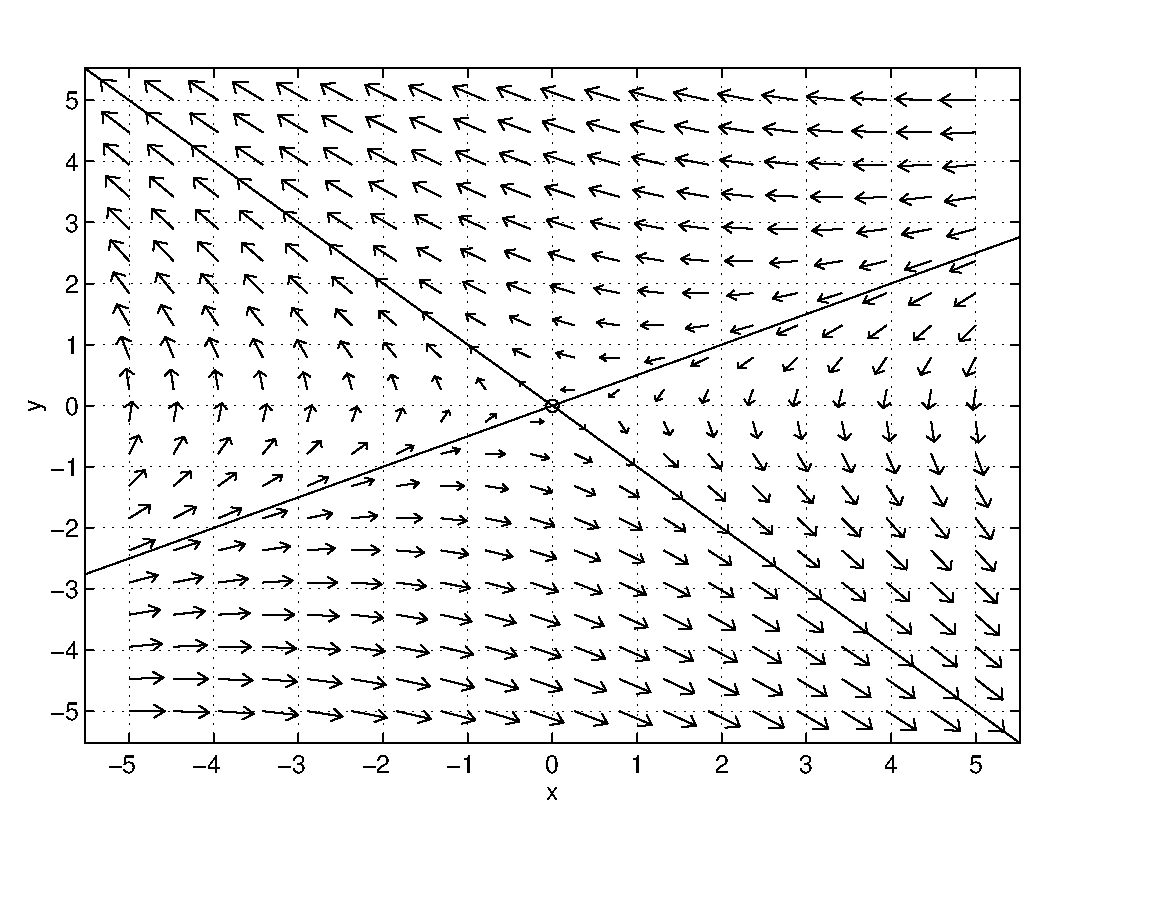
\psfig{file=exfigure/6-1-4a.eps,width=1.8in}
                       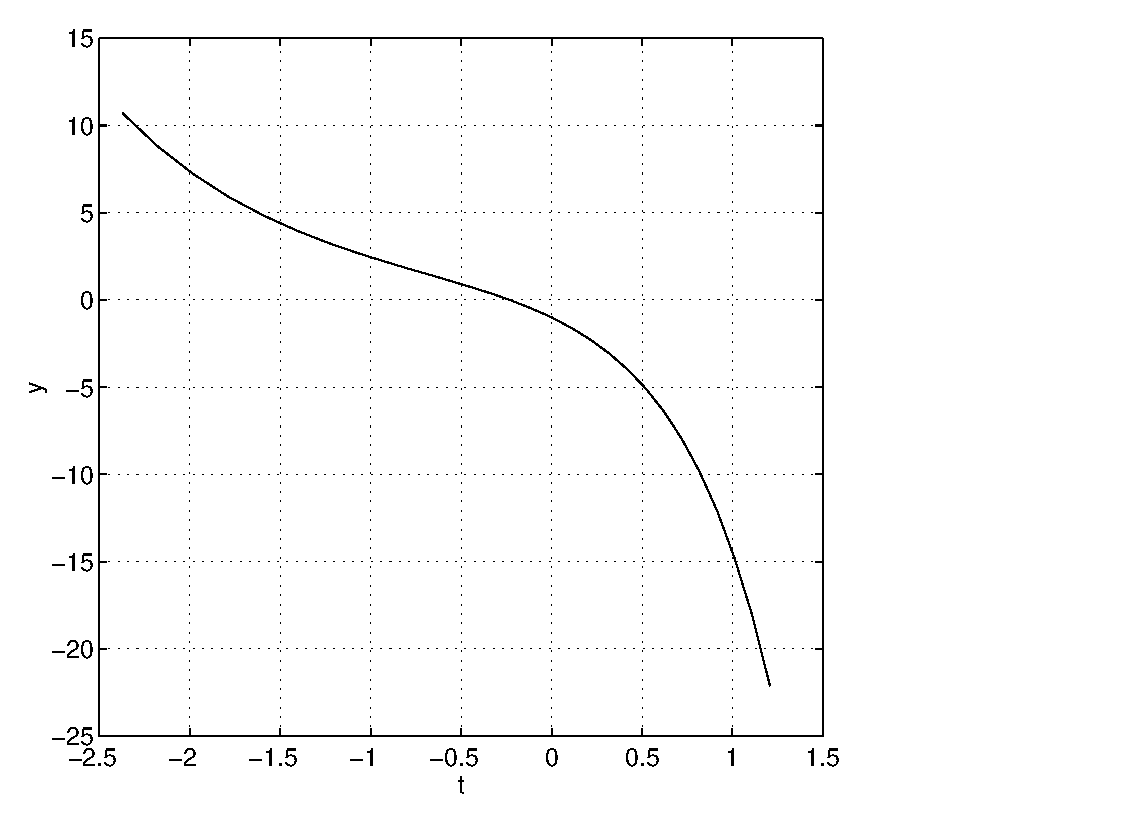
\psfig{file=exfigure/6-1-4b.eps,width=1.8in}
                       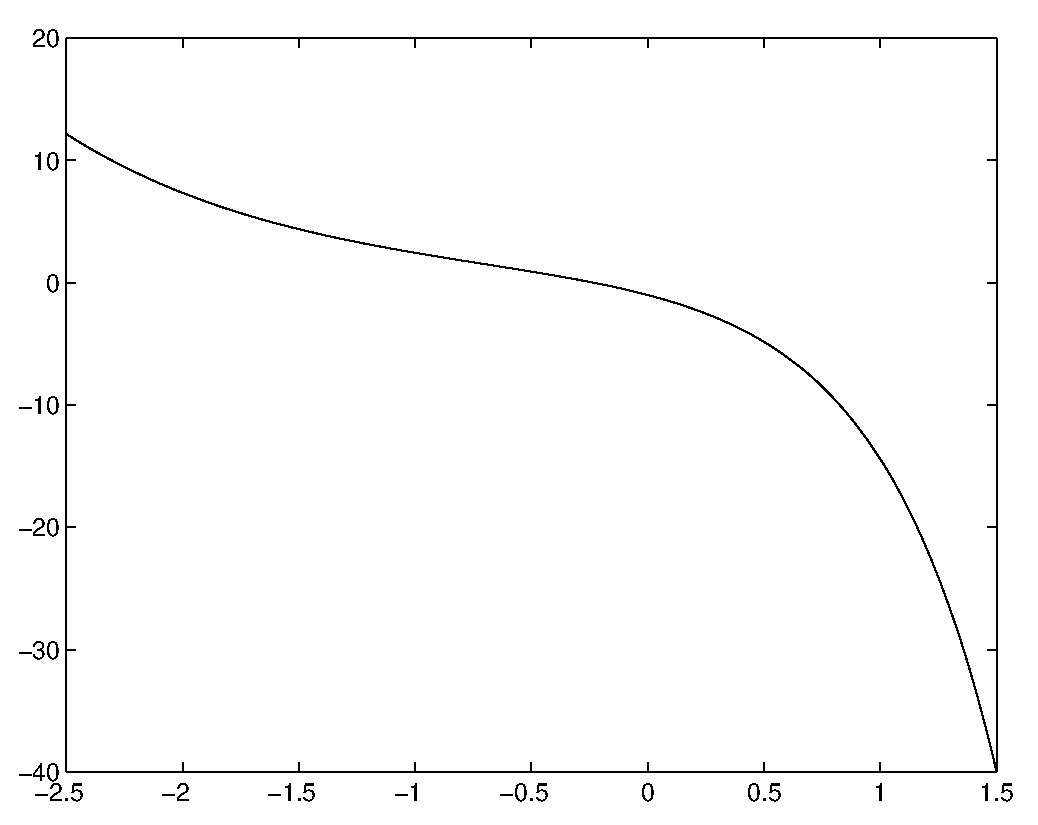
\psfig{file=exfigure/6-1-4c.eps,width=1.8in}}
                \exercapthree{c6.1.4}
\end{figure}



\subsection*{Section~\protect{\ref{S:TDM}} Closed Form Solutions by the Direct
Method}
\rhead{S:TDM}{CLOSED FORM SOLUTIONS BY THE DIRECT METHOD}

\exer{c6.6.05}
Using the identities $i^2 = -1$, $i^3 = -i$, and $i^4 = 1$, write
the Taylor series:
\[
\begin{array}{rcl}
e^{i\theta} & = & 1 + i\theta + \frac{1}{2!}(i\theta)^2 +
\frac{1}{3!}(i\theta)^3 + \frac{1}{4!}(i\theta)^4 +
\frac{1}{5!}(i\theta)^5 + \cdots \\
& = & 1 + i\theta - \frac{1}{2!}\theta^2 - \frac{1}{3!}i\theta^3 +
\frac{1}{4!}\theta^4 + \frac{1}{5!}i\theta^5 + \cdots \\
& = & (1 - \frac{1}{2!}\theta^2 + \frac{1}{4!}\theta^4 - \cdots)
+ i(\theta - \frac{1}{3!}\theta^3 + \frac{1}{5!}\theta^5 - \cdots) \\
& = & \cos\theta + i\sin\theta. \end{array}
\]

\exer{c6.6.1b}
\ans $\sin(3\theta) = 3\cos^2\theta\sin\theta - \sin^3\theta$.

\soln Calculate using Euler's formula and De Moivre's formula:
\[
\begin{array}{rcl}
\cos(3\theta) + i\sin(3\theta)
& = & e^{3i\theta} \\
& = & (e^{i\theta})^3 \\
& = & (\cos\theta + i\sin\theta)^3 \\
& = & (\cos^2\theta + 2i\cos\theta\sin\theta - \sin^2\theta)
(\cos\theta + i\sin\theta) \\
& = & \cos^3\theta + 3i\cos^2\theta\sin\theta -
3\sin^2\theta\cos\theta - i\sin^3\theta \\
& = & (\cos^3\theta - 3\sin^2\theta\cos\theta) +
i(3\cos^2\theta\sin\theta - \sin^3\theta).
\end{array}
\]
The imaginary part of this formula is equal to $\sin(3\theta)$.

\exer{c6.6.2b}
\ans The general solution to the differential equation is
\[
X(t) =
\alpha_1\cvectwo{5e^{2t}\cos(3t)}{e^{2t}(2\cos(3t) + \sin(3t))} +
\alpha_2\cvectwo{5e^{2t}\sin(3t)}{e^{2t}(2\sin(3t) - \cos(3t))}.
\]

\soln First, find the eigenvalues of $C$, which are the roots of the
characteristic polynomial
\[
p_C(\lambda) = \lambda^2 - 4\lambda + 13.
\]
The eigenvalues are $\lambda_1 = 2 + 3i$ and $\lambda_2 = 2 - 3i$.  Then,
find the eigenvector associated to $\lambda_1$ by solving the equation
\[
(C - \lambda_1I_2)v_1 =
\left(\mattwo{8}{-15}{3}{-4} - \cmattwo{2 + 3i}{0}{0}{2 + 3i}\right)v_1
= \cmattwo{6 - 3i}{-15}{3}{-6 - 3i}v_1 = 0.
\]
Solve this equation to find that
\[
v_1 = \cvectwo{5}{2 - i} = \vectwo{5}{2} + i\vectwo{0}{-1}
\]
is an eigenvector of $C$.  Since the eigenvalues of $C$ are complex, we
can find the general solution using \Ref{E:CC1} and \Ref{E:CC2}.  In this
case, since $\lambda_1 = 2 + 3i$ is
an eigenvalue, let $\sigma = 2$ and let $\tau = 3$.  Then $v_1 = v + iw$,
where $v = (5,2)^t$ and $w = (0,-1)^t$.  By \Ref{E:CC1},
\[
X_1(t) = e^{\sigma t}(\cos(\tau t)v - \sin(\tau t)w) \AND
X_2(t) = e^{\sigma t}(\sin(\tau t)v + \cos(\tau t)w)
\]
are solutions to the differential equation.  In this case,
\[
\begin{array}{rcl}
X_1(t) & = & e^{2t}\left(\cos(3t)\vectwo{5}{2} -
\sin(3t)\vectwo{0}{-1}\right)
= e^{2t}\cvectwo{5\cos(3t)}{\sin(3t) + 2\cos(3t)}. \\
X_2(t) & = & e^{2t}\left(\sin(3t)\vectwo{5}{2} +
\cos(3t)\vectwo{0}{-1}\right)
= e^{2t}\cvectwo{5\sin(3t)}{2\sin(3t) - \cos(3t)}.
\end{array}
\]
The general solution consists of all linear combinations
$X(t) = \alpha_1X_1(t) + \alpha_2X_2(t)$.

\exer{c6.6.2d} \ans The general solution to the differential equation is
\[
X(t) = \alpha e^{-2t}\cvectwo{2}{1} + \beta e^{-2t}\cvectwo{2t + 1}{t + 1}.
\]

\soln First, find the eigenvalues of $C$, which are the roots of the
characteristic polynomial
\[
p_C(\lambda) = \lambda^2 + 4\lambda + 4 = (\lambda + 2)^2.
\]
Thus, $C$ has a double eigenvalue at $\lambda_1 = -2$.  Since $C$ is not
a multiple of $I_2$, $C$ has only one linearly independent eigenvector.
Find this eigenvector by solving the equation
\[
(C - \lambda_1I_2)v_1 = \left(\mattwo{-4}{4}{-1}{0} + \mattwo{2}{0}{0}{2}
\right)v_1 = \mattwo{-2}{4}{-1}{2}v_1 = 0,
\]
obtaining $v_1 = (2,1)^t$.  Find the generalized eigenvector $w_1$ by
solving the equation $(C - \lambda_1 I_2)w_1 = v_1$, that is,
\[
\mattwo{-2}{4}{-1}{2}w_1 = \vectwo{2}{1}.
\]
So $w_1 = (1,1)^t$ is the generalized eigenvector.
Now, by \Ref{e:exp1eva}, we know that the
general solution to $\dot{X} = CX$ when $C$ has equal eigenvalues and only
one independent eigenvector is
\[
X(t) = e^{\lambda_1 t}(\alpha v_1 + \beta(w_1 + tv_1)).
\]
In this case,
\[
X(t) = e^{-2t}\left(\alpha \vectwo{2}{1} + \beta\left(\vectwo{1}{1} +
t\vectwo{2}{1}\right)\right).
\]



\subsection*{Section~\protect{\ref{S:Matrixexp}} Solutions Using Matrix
Exponentials}
\rhead{S:Matrixexp}{SOLUTIONS USING MATRIX EXPONENTIALS}

\exer{c6.2.1}
\ans When $m = 7$, the power series is accurate up to two decimal places.

\soln Enter {\tt L} into \Matlab, then use the command {\tt expm(L)} to
find the value of $e^L$.
\begin{verbatim}
ans = 
    4.8746         0   -3.9421
    3.1370    0.3679    2.4154
    3.9421         0    0.9324
\end{verbatim}
Then, add elements of the power series to $I_3$ until this answer is
is equal to the \Matlab generated answer up to a precision of two
digits.

\exer{c6.2.3}
One example of matrices for which $e^{C_1 + C_2} \neq e^{C_1}e^{C_2}$ is
\[ C_1 = \mattwo{1}{-2}{3}{1} \AND C_2 = \mattwo{-2}{3}{-1}{-2}. \]
For this case, using \Matlabp,
\begin{verbatim}
expm(C1+C2) =                        expm(C1)*expm(C2) =
    0.8013    0.5034                     0.1547   -0.4534
    1.0067    0.8013                     0.1152    0.5370
\end{verbatim}

\exer{c6.2.4b} \ans $e^{tC} =
\cmatthree{1}{t}{\frac{t^2}{2}}{0}{1}{t}{0}{0}{1}$.

\soln Since $D^3 = 0$,
\[
e^{tD} = I_3 + tD + \frac{t^2}{2}D^2 =
\matthree{1}{0}{0}{0}{1}{0}{0}{0}{1} +
\matthree{0}{t}{0}{0}{0}{t}{0}{0}{0} +
\cmatthree{0}{0}{\frac{t^2}{2}}{0}{0}{0}{0}{0}{0} =
\cmatthree{1}{t}{\frac{t^2}{2}}{0}{1}{t}{0}{0}{1}.
\]

\exer{c6.2.5}
By equation~\Ref{ex:expm}, $e^{\alpha I} = e^\alpha I$.  Therefore,
\[ e^{(\alpha + \beta)I} = e^{\alpha + \beta}I = e^\alpha e^\beta I
= e^\alpha I e^\beta I = e^{\alpha I}e^{\beta I}. \]

\exer{c6.2.5B}
(a) To verify that $Y(t)$ is a solution to the initial value problem
\Ref{E:init2}, first substitute $Y(t)$ into the left hand side of the
equation.  Using the chain rule, obtain
\[
\frac{dY}{dt}(t) = \frac{d}{dt}(e^{(t + s)A}X_0) =
\frac{d}{dt}((t + s)A)e^{(t + s)A}X_0 = Ae^{(t + s)A}X_0.
\]
Then substitute $Y(t)$ into the right hand side of the equation, obtaining
\[
AY(t) = Ae^{(t + s)A}X_0.
\]
Thus, the left hand and right hand sides of the equation are equal, so
$Y(t)$ is a solution to the differential equation.  Finally, check to see
that $Y(t)$ satisfies the initial value:
\[
Y(0) = e^{(0 + s)A}X_0 = e^{sA}X_0,
\]
as desired.

(b) Similarly, verify that $Z(t) = e^{tA}(e^{sA}X_0)$ is a solution to the
initial value problem by substituting $Z(t)$ into each side of the
differential equation:
\[
\frac{dZ}{dt}(t) = \frac{d}{dt}(e^{tA}(e^{sA}X_0))
= Ae^{tA}(e^{sA}X_0) \AND
AZ(t) = Ae^{tA}(e^{sA}X_0).
\]
Since the results are equal, $Z(t)$ is a solution to the differential
equation.  Evaluating at $t = 0$, we find
\[
Z(0) = e^{0}(e^{sA}X_0) = e^{sA}X_0,
\]
from which it follows that $Z(t)$ is also a solution to the initial
value problem.

(c) Since $Y(t)$ and $Z(t)$ are both solutions to the initial value problem
\[
\begin{array}{rcl}
\frac{dX}{dt} & = & AX \\
X(0) & = & e^{sA}X_0,
\end{array}
\]
it follows from the uniqueness part of Theorem~\ref{exist&unique} that
$Y(t) = Z(t)$.  Thus, $e^{(t + s)A} = e^{tA}e^{sA}$, as desired.

\exer{c6.2.6A} By Theorem~\ref{T:linODEsoln},
the unique solution to the differential equation $\dot{X} = CX$ with
initial condition $X(0) = X_0$ is $X(t) = e^{tC}X_0$.  Let $X(0) =
e_j$.  Then the vector $X_j(t) = e^{tC}e_j$ is a solution to the
differential equation, and is the $j^{th}$ column of the matrix
$e^{tC}$.  Thus, each column of $e^{tC}$ is a solution to the
differential equation, and the set of columns forms a basis of
solutions.

\exer{c6.2.8}
(a) Let $a_{ij}$ be the $(i,j)^{th}$ entry in $n \times n$ matrix $A$. 
Then, since $|a_{ij}| \geq 0$ for all $(i,j)$,
\[ |a_{ij}| \leq |a_{i1}| + \cdots + |a_{in}| \leq
\max_i(|a_{i1}| + \cdots + |a_{in}|) = ||A||_m. \]
This statement is valid for the matrix $A^N$, so $|a_N| \leq ||A^N||_m$.

(b) To show this, we use the fact that $||A^N||_m = ||A^{N - 1}A||_m$.
According to Exercise~\ref{c6.2.7},
\[
||A^{N - 1}A||_m \leq ||A^{N - 1}||_m ||A||_m.
\]
Expanding $||A^N||_m$ in this way, we find that
\[
||A^N||_m \leq ||A||_m \cdots ||A||_m = ||A||^N_m.
\]

(c) According to our result in (a)
\[ |a_0| + |a_1| + \cdots + \frac{1}{N!}|a_N| = \sum_N
\frac{1}{N!}|a_N| \leq \sum_N \frac{1}{N!}||A^N||_m. \]
According to the result in (b)
\[ \sum_N \frac{1}{N!}||A^N||_m \leq \sum_N \frac{1}{N!}||A||^N_m. \]
We know that
\[ \sum_{N = 0}^{\infty} \frac{1}{N!}||A||^N_m = e^{||A||_m}.  \]
Therefore,
\[ \sum_N \frac{1}{N!}|a_N| \leq e^{||A||_m}, \]
so $e^A$ is absolutely convergent.



\subsection*{Section~\protect{\ref{S:LNFPS}} Linear Normal Form Planar Systems}
\rhead{S:LNFPS}{LINEAR NORMAL FORM PLANAR SYSTEMS}

\exer{c6.3.1}
\ans The solution to the initial value problem $(x(0),y(0) = (1,-2)$ for
this system is:
\[
\vectwo{x(t)}{y(t)} = \vectwo{e^{2t}(\cos(3t) - 2\sin(3t))}
{-e^{2t}(\sin(3t) + 2\cos(2t))}.
\]

\soln Let $\sigma = 2$ and $\tau = -3$.  Then,
\[
\begin{array}{rrr}
\dot{x} & = & \sigma x - \tau y \\
\dot{y} & = & \tau x + \sigma y \end{array}
\]
so, according to Table~\ref{T:3sys}
\[
\vectwo{x(t)}{y(t)} = \vectwo{e^{\sigma t}(x_0\cos(\tau t) -
y_0\sin(\tau t))}{e^{\sigma t}(x_0\sin(\tau t) +
y_0\cos(\tau t))} = \vectwo{e^{2t}(x_0\cos(-3t) - y_0\sin(-3t))}
{e^{2t}(x_0\sin(-3t) + y_0\cos(2t))}.
\]

\exer{c6.3.25}
\ans $e^{tC} = e^{2t}(I_n + tA + \frac{t^2}{2}A^2)$.

\soln Since $(2I)A = A(2I)$, we can use Proposition~\ref{P:expAB} to
show that
\[
e^{tC} = e^{t(2I_n + A)} = e^{2tI_n}e^{tA}.
\]
Then, since $A^3 = 0$,
\[
e^{2tI_n}e^{tA} = e^{2t}I_n(I_n + tA + \frac{t^2}{2}A^2).
\]



\subsection*{Section~\protect{\ref{S:6.5}} Similar Matrices}
\rhead{S:6.5}{SIMILAR MATRICES}

\exer{c6.5.1}
Since $A$ and $B$ are similar and $B$ and $C$ are similar,
$A = P^{-1}BP$ for some matrix $P$, and $B = Q^{-1}BQ$
for some matrix $Q$.  Therefore,
\[ A = P^{-1}BP = P^{-1}Q^{-1}CQP. \]
By Proposition~\ref{P:invprod}, $(QP)^{-1} = P^{-1}Q^{-1}$, so
\[ A = (QP)^{-1}C(QP) \]
thus, $A$ and $C$ are similar.

\exer{c6.5.3a}
\ans Matrices $A$ and $B$ are not similar.

\soln When two matrices are similar, the traces are equal.  In this case,
$\trace(A) = 5$ and $\trace(B) = 10$, so the matrices are not similar.

\exer{c6.5.4}
Since, $A$ and $B$ are similar matrices, if $Bv = \lambda v$, then
\[ A(Pv) = PP^{-1}APv = PBv = \lambda (Pv). \]
Thus, $Pv$ is an eigenvector of $A$ with eigenvalue $\lambda$.

\exer{c6.5.6}
\ans $\dps e^A = e^2\mattwo{2}{-1}{1}{0}$.

\soln We cannot compute $e^A$ directly by hand.  By Lemma~\ref{L:similarexp},
if $B = P^{-1}AP$, then $e^B = P^{-1}e^AP$.  Therefore, we solve by
finding a matrix similar to $A$ whose exponential can be computed.  
We first find the eigenvalues of $A$ and associated eigenvectors.
If $\lambda$ is an eigenvalue of $A$, then $\det(A - \lambda I_2) =
0$, or, since $A$ is a $2 \times 2$ matrix,
\[ 0 = \lambda^2 - \trace(A)\lambda + det(A) = \lambda^2 - 4\lambda +
4 = (\lambda - 2)^2. \]
Thus, $A$ has one eigenvalue, $\lambda = 2$.  To find the associated
eigenvector, solve $(A - \lambda I_2)v = 0$ by row reduction:
\[ A - 2I_2 = \mattwo{1}{-1}{1}{-1} \longrightarrow
\mattwo{1}{-1}{0}{0}. \]
So, $v = (1,1)$ is an eigenvector of $A$ associated to $\lambda$.
By Theorem~\ref{T:putinform}, since $A$
has one real eigenvector, 
\[ B = \mattwo{\lambda}{1}{0}{\lambda} = \mattwo{2}{1}{0}{2} \]
is a matrix similar to $A$.  We can then compute $P = (v|w)$, where
$Aw = v + \lambda w$, that is, $(A - \lambda I_2)w = v$.  We can solve
by row reducing the augmented matrix $(A - \lambda I_2|v)$:
\[ \left(\begin{array}{rr|r} 1 & -1 & 1 \\ 1 & -1 & 1 \end{array}
\right) \longrightarrow \left(\begin{array}{rr|r} 1 & -1 & 1 \\
0 & 0 & 0 \end{array}\right). \]
Thus, $w = (2,1)$, so
\[ P = \mattwo{1}{2}{1}{1} \]
and $A$ and $B$ are similar.
We now compute $e^A = Pe^BP^{-1}$.  Using \Ref{e:expshear},
\[ e^B = e^2\mattwo{1}{1}{0}{1}. \]
So we calculate 
\[ e^A = Pe^BP^{-1} = \mattwo{1}{2}{1}{1}e^2\mattwo{1}{1}{0}{1}
\mattwo{-1}{2}{1}{-1} = e^2\mattwo{2}{-1}{1}{0}. \]



\subsection*{Section~\protect{\ref{S:6.6}} *Formulas for Matrix Exponentials}
\rhead{S:6.6}{*FORMULAS FOR MATRIX EXPONENTIALS}

\exer{c6.6.2}
\ans The solution to the given initial value problem with $X(0) = (2,1)^t$
is
\[
X(t) = -3e^t\vectwo{1}{1} + e^{2t}\vectwo{1}{2}
= \cvectwo{e^{2t} - 3e^t}{2e^{2t} - 3e^t}.
\]

\soln Let \[ C = \mattwo{0}{1}{-2}{3}. \]
Then the solution to the system is $X(t) = e^{tC}X_0$, where
$X_0 = X(0) = (2,1)^t$.
To find $e^{tC}$, first find the eigenvalues of $C$ by solving
\[
0 = \lambda^2 - \trace(C) + \det(C) = (\lambda - 1)(\lambda - 2).
\]
The eigenvalues are $\lambda_1 = 1$ and $\lambda_2 = 2$.  We can
then find $e^{tC}$ using \Ref{E:exdist}:
\[
\begin{array}{rcl}
e^{tC} & = & \frac{1}{\lambda_2 - \lambda_1}(e^{\lambda_1 t}(C -
\lambda_2 I_2) - e^{\lambda_2 t}(C - \lambda_1 I_2)) \\
& = & e^t\left(\mattwo{0}{1}{-2}{3} - \mattwo{2}{0}{0}{2}\right) -
e^{2t}\left(\mattwo{0}{1}{-2}{3} - \mattwo{1}{0}{0}{1}\right) \\
& = &
e^t\mattwo{-2}{1}{-2}{1} - e^{2t}\mattwo{-1}{1}{-2}{2}.
\end{array}
\]
So, we can now compute
\[
X(t) = e^{tC}X_0
= \left(e^t\mattwo{-2}{1}{-2}{1} -
e^{2t}\mattwo{-1}{1}{-2}{2}\right)\vectwo{2}{1}.
\]
Complete the matrix multiplication to obtain $X(t)$.

\exer{c6.6.4}
\ans The solution to the initial value problem $X(0) = (1,1)^t$ is:
\[
X(t) = e^t\vectwo{2\sin{t} + \cos{t}}{-3\sin{t} + \cos{t}}.
\]

\soln Let
\[
C = \mattwo{2}{1}{-2}{0}.
\]
Then the solution to the system is $X(t) = e^{tC}X_0$, where
$X_0 = X(0)$ is the initial condition of the system.
Find the eigenvalues of $C$ by solving
\[
0 = \lambda^2 - \trace(C) + \det(C) = \lambda^2 - 2\lambda + 2.
\]
So the eigenvalues of $C$ are $\lambda_1 = 1 + i$ and $\lambda_2 = 1 - i$.
We can then find $e^{tC}$ using 
\Ref{E:exdist}:
\[
e^{tC} = \frac{1}{\lambda_2 - \lambda_1}(e^{\lambda_1 t}(C -
\lambda_2 I_2) - e^{\lambda_2 t}(C - \lambda_1 I_2)).
\]
Since the scalar
\[
\frac{1}{\lambda_2 - \lambda_1} = -\frac{1}{2}i
\]
is purely imaginary, we need compute only the imaginary parts of
$e^{\lambda_1 t}(C - \lambda_2 I_2)$ and $e^{\lambda_2 t}(C - \lambda_1 I_2)$
to obtain the real solution to the differential equation $X(t) = e^{tC}X_0$.
So, compute
\[
\begin{array}{rcl}
e^{\lambda_1 t}(C - \lambda_2 I_2)
& = & e^{t}e^{it}\left(\mattwo{2}{1}{-2}{0} - \cmattwo{1 - i}{0}{0}{1 - i}
\right) \\
& = & e^{t}(\cos t + i\sin t)\cmattwo{1 + i}{1}{-2}{-1 + i}.
\end{array}
\]
The imaginary part of this product is
\[
ie^t\cmattwo{\sin t + \cos t}{\sin t}{-2\sin t}{-\sin t + \cos t}.
\]
Then compute
\[
\begin{array}{rcl}
e^{\lambda_2 t}(C - \lambda_1 I_2)
& = & e^{t}e^{-it}\left(\mattwo{2}{1}{-2}{0} - \cmattwo{1 + i}{0}{0}{1 + i}
\right) \\
& = & e^{t}(\cos t - i\sin t)\cmattwo{1 - i}{1}{-2}{-1 - i}.
\end{array}
\]
The imaginary part of this product is
\[
ie^t\cmattwo{-\sin t - \cos t}{-\sin t}{2\sin t}{\sin t - \cos t}.
\]
Thus, the solution to the given initial value problem is
\[
X(t) = e^{tC}X_0 =
\frac{1}{2}\cmattwo{2\sin t + 2\cos t}{2\sin t}{-4\sin t}{-2\sin t + 2\cos t}
\vectwo{1}{0}.
\]
Complete the matrix multiplication to obtain $X(t)$.



\subsection*{Section~\protect{\ref{S:SOE}} Second Order Equations}
\rhead{S:SOE}{SECOND ORDER EQUATIONS}

\exer{c6.7.1}
\ans The particle will hit the ground at $t \approx 1.63$ seconds.

\soln Let $g(t) = 32$.  Then integrate:
\[
\begin{array}{rcl}
\frac{d^2x}{dt^2} & = & -g \\
\frac{dx}{dt} & = & \int (-g)dt \\
\frac{dx}{dt} & = & -32t + v_0 \\
x & = & \int (-32t + C_1)dt \\
x & = & -16t^2 + C_1t + C_2.
\end{array}
\]
Then let $C_1 = v_0$, the initial velocity, and let $C_2 = x_0$, the initial
position of the particle, to obtain $x(t) = -16t^2 + v_0t + x_0$.  In this
case, $x(t) = -16t^2 + 20t + 10$.  Solve for $x(t) = 0$ to find
$t = \frac{10 + \sqrt{260}}{16} \approx 1.63$.

\exer{c6.6.hoa}
\ans The general solution is
\[
x(t) = \alpha e^t + \beta e^{-3t}
\]
for $\alpha, \beta \in \R$.

\soln Let $y = \dot{x}$, and rewrite the differential equation as
$\dot{y} + 2y - 3x = 0$.  Write the first order system in two equations:
\[
\begin{array}{rrrrr}
\dot{x} & = & & & y \\
\dot{y} & = & 3x & - & 2y.
\end{array}
\]
This system can be represented by the matrix $Q$, where
\[
Q = \mattwo{0}{1}{3}{-2}.
\]
The characteristic polynomial of $Q$ is $p_Q(\lambda) = \lambda^2
+ 2\lambda - 3$, and the eigenvalues are $\lambda_1 = 1$ and
$\lambda_2 = 2$.  Thus, the general solution is
\[
x(t) = \alpha e^{\lambda_1t} + \beta e^{\lambda_2t} =
\alpha e^t + \beta e^{-3t}.
\]

\exer{c6.6.hoc}
\ans The general solution is
\[
x(t) = e^{-t}(\alpha \cos{t} + \beta \sin{t}).
\]

\soln Let $y \dot{x}$ and rewrite the system as $\dot{y} + 2y + 2x = 0$,
or $\dot{X} = QX$, where
\[
X = \vectwo{x}{y} \AND Q = \mattwo{0}{1}{-2}{-2}.
\]
The characteristic polynomial of $Q$ is $p_q(\lambda) = \lambda^2 
+ 2\lambda + 2$, and the eigenvalues of $Q$ are $\lambda_1 = -1 + i$ and
$\lambda_2 = -1 - i$.  Thus, the general solution is
\[
x(t) = c_1e^{(-1 + i)t} + c_2e^{(-1 - i)t}
\]
for some $c_1, c_2 \in \C$.  Using Euler's formula $e^{i\theta} =
\cos\theta + i\sin\theta$, we can write
\[
\begin{array}{rcl}
x(t) & = & c_1e^{-t}e^{it} + c_2e^{-t}e^{-it} \\
& = & e^{-t}(c_1(\cos{t} + i\sin{t}) + c_2(\cos{t} - i\sin{t})) \\
& = & e^{-t}((c_1 + c_2)\cos{t} + i(c_1 - c_2)\sin{t}).
\end{array}
\]
We know that $x(t) \in \R$ for all $t$.  Thus, $(c_1 + c_2) \in \R$, and
$(c_1 - c_2)$ is purely imaginary, so $c_2 = \overline{c_1}$.  Let
$c_1 = \frac{1}{2}(\alpha + i\beta)$ for $\alpha, \beta \in \R$. 
Then $x(t) = e^{-t}(\alpha\cos{t} + \beta\sin{t})$.

\exer{c6.7.4}
This differential equation can be rewritten as $\dot{X} = QX$, where
$y = \dot{x}$,
\[
X = \vectwo{x}{y}, \AND Q = \mattwo{0}{1}{-w}{-r}.
\]
Then we can solve for $x(t)$ in closed form, obtaining
\[
x(t) = \alpha e^{\lambda_1 t} + \beta e^{\lambda_2 t}
\]
where $\lambda_1$ and $\lambda_2$ are the roots of the characteristic
polynomial $p_q(\lambda) = \lambda^2 + r\lambda + w$.  By the quadratic
formula, the eigenvalues are
\[
\lambda = \frac{-r \pm \sqrt{r^2 - 4w}}{2}.
\]
We know that $-r < 0$.  If $r^2 - 4w < 0$, then $\lambda_1$ and $\lambda_2$
are complex conjugates with negative real part.  Otherwise, $\lambda_1$
and $\lambda_2$ are negative real numbers, since $r > \sqrt{r^2 - 4w}$
for any choice of $r$ and $w$.  For any $\lambda$ with negative real part
\[
\lim_{t \rightarrow \infty} e^{\lambda t} = 0.
\]
Thus,
\[
\lim_{t \rightarrow \infty} x(t) =
\lim_{t \rightarrow \infty} (\alpha e^{\lambda_1 t} +
\beta e^{\lambda_2 t}) = 0.
\]

\exer{c6.6.tfb} \ans False.

\soln As a counterexample, consider the trivial case in which $x(t)$
is identically $0$.

\exer{c3.5.5}
Let $x(t)$ be a solution to the second order differential equation
\begin{equation} \label{order2}
\frac{d^2x}{dt^2} + a(x)\frac{dx}{dt} + b(x) = 0.
\end{equation}
Let $y(t) = \dot x(t)$.  Then \Ref{order2} can be rewritten as
\[ \frac{d}{dt}\left(\frac{dx}{dt}\right) + a(x)\frac{dx}{dt}
+ b(x) = \frac{dy}{dt} + a(x)y + b(x) = 0 \]
So any solution to \Ref{order2} is also a solution to the system
\begin{equation} \label{order2sol}
\begin{array}{rcl}
\dot{x} & = & y \\
\dot{y} & = & -b(x) - a(x) y.\end{array}
\end{equation}
Conversely, we can solve system \Ref{order2sol} as follows
\[ \begin{array}{rcl}
\frac{d}{dx}\left(\dot{x}\right) & = & -b(x) - a(x)\dot{x} \\
\frac{d^2x}{dt^2} & = & -b(x) - a(x)\frac{dx}{dt}\end{array}
\]
to show that any solution to \Ref{order2sol} is also a solution
to \Ref{order2}.






















\end{document}
